% --------------------------------------------------
% 
% This chapter is for HPC
% 
% --------------------------------------------------

\chapter{0s and 1s in marine molecular research}
\label{cha:hpc}


Publication relative to this chapter: \cite{zafeiropoulos20210s}


\section{Computing resources: a  prerequisite \& a limitation in modern microbial ecology}




\begin{figure}{}
   \centering
   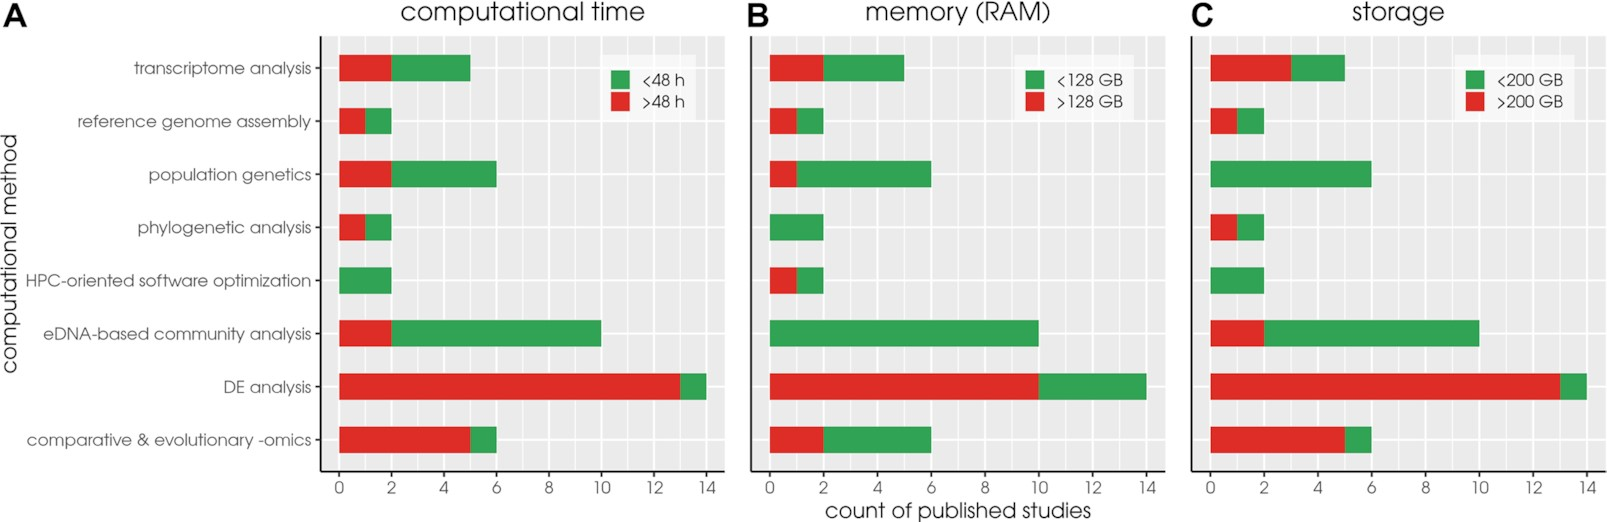
\includegraphics[width=140mm]{figures/zorbas_jobs_resources.jpeg}
   \caption{Computing requirements of the published studies performed on the IMBBC HPC facility over the last decade. Figure from publication.
   % Red bars denote published research with high resource requirements of the various computational methods employed at the IMBBC HPC facility due to (a) long computational times (>48 h), (b) high memory requirements (>128 GB), or (c) high storage requirements (>200 GB). For instance, no eDNA-based community analyses performed at Zorba thus far have required a large amounts of memory.
   }
   \label{fig:zorba_jobs}
\end{figure}


\section{High Performance Computing and Cloudification: scaling up bioinformatics analysis}



